\documentclass{beamer}

%
% Common preamble for all three parts.
%
\usepackage[utf8]{inputenc}
\usepackage[ngerman]{babel}
\usepackage{amsmath}
\usepackage{color}
\usepackage{minted}
\usepackage{hyperref}
\usepackage{multicol}
\usepackage{tabularx}
\usepackage{tikz}

% only inline todonotes work
\usepackage{xkeyval}
\usepackage[textsize=small]{todonotes}
\presetkeys{todonotes}{inline}{}

\usetikzlibrary{shapes,arrows,positioning,shadows}

% no nav buttons
\usenavigationsymbolstemplate{}

\newcommand{\bftt}[1]{\textbf{\texttt{#1}}}
\newcommand{\comment}[1]{{\color[HTML]{008080}\textit{\textbf{\texttt{#1}}}}}
\newcommand{\cmd}[1]{{\color[HTML]{008000}\bftt{#1}}}
\newcommand{\bs}{\char`\\}
\newcommand{\cmdbs}[1]{\cmd{\bs#1}}
\newcommand{\lcb}{\char '173}
\newcommand{\rcb}{\char '175}
\newcommand{\cmdbegin}[1]{\cmdbs{begin\lcb}\bftt{#1}\cmd{\rcb}}
\newcommand{\cmdend}[1]{\cmdbs{end\lcb}\bftt{#1}\cmd{\rcb}}

\newcommand{\wllogo}{\textbf{Overleaf}}

% this is where the example source files are loaded from
% do not include a trailing slash
\newcommand{\fileuri}{https://raw.github.com/stefan-mueller/latex-course/master/de}

\newcommand{\wlserver}{https://www.overleaf.com}
\newcommand{\wlnewdoc}[1]{\wlserver/docs?snip\_uri=\fileuri/#1\&splash=none}

\def\tikzname{Ti\emph{k}Z}

% from http://tex.stackexchange.com/questions/5226/keyboard-font-for-latex
\newcommand*\keystroke[1]{%
  \tikz[baseline=(key.base)]
    \node[%
      draw,
      fill=white,
      drop shadow={shadow xshift=0.25ex,shadow yshift=-0.25ex,fill=black,opacity=0.75},
      rectangle,
      rounded corners=2pt,
      inner sep=1pt,
      line width=0.5pt,
      font=\scriptsize\sffamily
    ](key) {#1\strut}
  ;
}
\newcommand{\keystrokebftt}[1]{\keystroke{\bftt{#1}}}

% stolen from minted.dtx
\newenvironment{exampletwoup}
  {\VerbatimEnvironment
   \begin{VerbatimOut}{example.out}}
  {\end{VerbatimOut}
   \setlength{\parindent}{0pt}
   \fbox{\begin{tabular}{l|l}
   \begin{minipage}{0.55\linewidth}
     \inputminted[fontsize=\small,resetmargins]{latex}{example.out}
   \end{minipage} &
   \begin{minipage}{0.35\linewidth}
     \input{example.out}
   \end{minipage}
   \end{tabular}}}

\newenvironment{exampletwouptiny}
  {\VerbatimEnvironment
   \begin{VerbatimOut}{example.out}}
  {\end{VerbatimOut}
   \setlength{\parindent}{0pt}
   \fbox{\begin{tabular}{l|l}
   \begin{minipage}{0.55\linewidth}
     \inputminted[fontsize=\scriptsize,resetmargins]{latex}{example.out}
   \end{minipage} &
   \begin{minipage}{0.35\linewidth}
     \setlength{\parskip}{6pt plus 1pt minus 1pt}%
     \raggedright\scriptsize\input{example.out}
   \end{minipage}
   \end{tabular}}}

\newenvironment{exampletwouptinynoframe}
  {\VerbatimEnvironment
   \begin{VerbatimOut}{example.out}}
  {\end{VerbatimOut}
   \setlength{\parindent}{0pt}
   \begin{tabular}{l|l}
   \begin{minipage}{0.55\linewidth}
     \inputminted[fontsize=\scriptsize,resetmargins]{latex}{example.out}
   \end{minipage} &
   \begin{minipage}{0.35\linewidth}
     \setlength{\parskip}{6pt plus 1pt minus 1pt}%
     \raggedright\scriptsize\input{example.out}
   \end{minipage}
   \end{tabular}}

\title{Eine interaktive Einführung in \LaTeX}
\author{Stefan Müller}
\titlegraphic{%

\includegraphics[height=36pt]{overleaf}\\[1em]

\includegraphics[height=24pt]{tcd-logo}
}


\subtitle{Teil 1: Grundlagen \\ 
(\href{https://github.com/jdleesmiller/latex-course}{basierend auf den Folien von Dr. John D. Lees-Miller})}

\begin{document}

%%%%%%%%%%%%%%%%%%%%%%%%%%%%%%%%%%%%%%%%%%%%%%%%%%%%%%%%%%%%%%%%%%%%%%%%%%%%%%%
%%%%%%%%%%%%%%%%%%%%%%%%%%%%%%%%%%%%%%%%%%%%%%%%%%%%%%%%%%%%%%%%%%%%%%%%%%%%%%%
%%%%%%%%%%%%%%%%%%%%%%%%%%%%%%%%%%%%%%%%%%%%%%%%%%%%%%%%%%%%%%%%%%%%%%%%%%%%%%%
\begin{frame}
\titlepage
\end{frame}

%%%%%%%%%%%%%%%%%%%%%%%%%%%%%%%%%%%%%%%%%%%%%%%%%%%%%%%%%%%%%%%%%%%%%%%%%%%%%%%
%%%%%%%%%%%%%%%%%%%%%%%%%%%%%%%%%%%%%%%%%%%%%%%%%%%%%%%%%%%%%%%%%%%%%%%%%%%%%%%
%%%%%%%%%%%%%%%%%%%%%%%%%%%%%%%%%%%%%%%%%%%%%%%%%%%%%%%%%%%%%%%%%%%%%%%%%%%%%%%
\begin{frame}{Warum \LaTeX{}?}
\begin{itemize}
\item Es erstellt wunderschöne Dokumente
\begin{itemize}
\item Insbesondere mathematische Formeln
\end{itemize}
%
\item Erstellt von Wissenschaftlern für Wissenschaftler 
\begin{itemize}
\item Eine große und aktive Community
\end{itemize}
%
\item Es ist leistungsfähig -- und Du kannst es erweiteren
\begin{itemize}
\item Erweiterungen für Papers, Präsentationen, Poster, Lebensläufe, \ldots
\end{itemize}
\end{itemize}
\end{frame}

%%%%%%%%%%%%%%%%%%%%%%%%%%%%%%%%%%%%%%%%%%%%%%%%%%%%%%%%%%%%%%%%%%%%%%%%%%%%%%%
%%%%%%%%%%%%%%%%%%%%%%%%%%%%%%%%%%%%%%%%%%%%%%%%%%%%%%%%%%%%%%%%%%%%%%%%%%%%%%%
%%%%%%%%%%%%%%%%%%%%%%%%%%%%%%%%%%%%%%%%%%%%%%%%%%%%%%%%%%%%%%%%%%%%%%%%%%%%%%%
\begin{frame}[fragile]{Wie funktioniert \LaTeX?}
\begin{itemize}
\item Schreibe das Dokument in \texttt{plain text} mit \cmd{Befehlen}, die 
die Struktur und Bedeutung definieren. 
\item \texttt{latex} verarbeitetet den Text und die Befehle
und erstellt wundervoll formatierte Dokumente.
\end{itemize}
\vskip 2ex
\begin{center}
\begin{minted}[frame=single]{LaTeX}
\LaTeX{} ist ein \emph{hilfreiches} Programm.
\end{minted}
\vskip 2exh
\tikz\node[single arrow,fill=gray,font=\ttfamily\bfseries,%
  rotate=270,xshift=-1em]{latex};
\vskip 2ex
\fbox{\LaTeX{} ist ein \emph{hilfreiches} Programm.}
\end{center}
\end{frame}

%%%%%%%%%%%%%%%%%%%%%%%%%%%%%%%%%%%%%%%%%%%%%%%%%%%%%%%%%%%%%%%%%%%%%%%%%%%%%%%
%%%%%%%%%%%%%%%%%%%%%%%%%%%%%%%%%%%%%%%%%%%%%%%%%%%%%%%%%%%%%%%%%%%%%%%%%%%%%%%
%%%%%%%%%%%%%%%%%%%%%%%%%%%%%%%%%%%%%%%%%%%%%%%%%%%%%%%%%%%%%%%%%%%%%%%%%%%%%%%
\begin{frame}[fragile]{Weitere Beispiele für Befehle und deren Ergebnis\ldots}
\begin{exampletwoup}
\begin{itemize}
\item Tee
\item Milch
\item Kekse
\end{itemize}
\end{exampletwoup}
\vskip 2ex
\begin{exampletwoup}
\begin{figure}
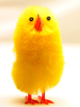
\includegraphics{kueken}
\end{figure}
\end{exampletwoup}
\vskip 2ex
\begin{exampletwoup}
\begin{equation}
\alpha + \beta + 1
\end{equation}
\end{exampletwoup}

\tiny{Bild basierend auf \url{http://www.andy-roberts.net/writing/latex/importing_images}.}
\end{frame}

%%%%%%%%%%%%%%%%%%%%%%%%%%%%%%%%%%%%%%%%%%%%%%%%%%%%%%%%%%%%%%%%%%%%%%%%%%%%%%%
%%%%%%%%%%%%%%%%%%%%%%%%%%%%%%%%%%%%%%%%%%%%%%%%%%%%%%%%%%%%%%%%%%%%%%%%%%%%%%%
%%%%%%%%%%%%%%%%%%%%%%%%%%%%%%%%%%%%%%%%%%%%%%%%%%%%%%%%%%%%%%%%%%%%%%%%%%%%%%%
\begin{frame}[fragile]{Anpassung der Grundhaltung}

\begin{itemize}
\item Nutze die Befehle, um zu beschrieben „was ist“, nicht „wie es aussieht“.
\item Fokussiere Dich auf den Inhalt.
\item Lass \LaTeX{} den Rest machen.
\end{itemize}
\end{frame}

%%%%%%%%%%%%%%%%%%%%%%%%%%%%%%%%%%%%%%%%%%%%%%%%%%%%%%%%%%%%%%%%%%%%%%%%%%%%%%%
%%%%%%%%%%%%%%%%%%%%%%%%%%%%%%%%%%%%%%%%%%%%%%%%%%%%%%%%%%%%%%%%%%%%%%%%%%%%%%%
%%%%%%%%%%%%%%%%%%%%%%%%%%%%%%%%%%%%%%%%%%%%%%%%%%%%%%%%%%%%%%%%%%%%%%%%%%%%%%%
\section{Die Grundlagen}

%%%%%%%%%%%%%%%%%%%%%%%%%%%%%%%%%%%%%%%%%%%%%%%%%%%%%%%%%%%%%%%%%%%%%%%%%%%%%%%
%%%%%%%%%%%%%%%%%%%%%%%%%%%%%%%%%%%%%%%%%%%%%%%%%%%%%%%%%%%%%%%%%%%%%%%%%%%%%%%
%%%%%%%%%%%%%%%%%%%%%%%%%%%%%%%%%%%%%%%%%%%%%%%%%%%%%%%%%%%%%%%%%%%%%%%%%%%%%%%
\subsection{Erste Schritte}
\begin{frame}[fragile]{\insertsubsection}
\begin{itemize}
\item Ein Minimalbeispiel:
\inputminted[frame=single]{latex}{basics.tex}
\item Befehle starten mit einem \emph{Backslash} \keystrokebftt{\bs}.
\item Jedes Dokument beginnt mit einem \cmdbs{documentclass}-Befehl.
\item Ein \emph{Argument} in geschweiften Klammern \keystrokebftt{\{} \keystrokebftt{\}} zeigt \LaTeX{}, 
welche Art von Dokument es erstellen soll: in diesem Fall einen Artikel (\bftt{article}).
\item Ein Prozentzeichen \keystrokebftt{\%} startet einen \emph{Kommentar} --- \LaTeX{}
ignoriert den Rest der Zeile.
\end{itemize}
\end{frame}

%%%%%%%%%%%%%%%%%%%%%%%%%%%%%%%%%%%%%%%%%%%%%%%%%%%%%%%%%%%%%%%%%%%%%%%%%%%%%%%
%%%%%%%%%%%%%%%%%%%%%%%%%%%%%%%%%%%%%%%%%%%%%%%%%%%%%%%%%%%%%%%%%%%%%%%%%%%%%%%
%%%%%%%%%%%%%%%%%%%%%%%%%%%%%%%%%%%%%%%%%%%%%%%%%%%%%%%%%%%%%%%%%%%%%%%%%%%%%%%
\begin{frame}[fragile]{\insertsubsection{} mit \wllogo}
\begin{itemize}
\item Overleaf ist eine Website zur Erstellung von Dokumenten in \LaTeX.
\item Es kompiliert Dein Dokument automatisch und zeigt Dir das Resultat.
\vskip 2em
\begin{center}
\fbox{\href{\wlnewdoc{basics.tex}}{%
Klicke hier, um ein Beispiel-Dokument in \wllogo{} zu öffnen}}
\\[1ex]\scriptsize{}
\href{http://www.google.com/chrome}{Google Chrome} oder eine neuere Version von \href{http://www.mozilla.org/en-US/firefox/new/}{Firefox} garantieren die besten Ergebnisse.
\end{center}
\vskip 2ex
\item Während wir durch die Folien gehen, probiere die Beispiele in Overleaf aus.
\item \textbf{Wirklich, Du solltest die Befehle selber durchführen!}
\end{itemize}
\end{frame}

%%%%%%%%%%%%%%%%%%%%%%%%%%%%%%%%%%%%%%%%%%%%%%%%%%%%%%%%%%%%%%%%%%%%%%%%%%%%%%%
%%%%%%%%%%%%%%%%%%%%%%%%%%%%%%%%%%%%%%%%%%%%%%%%%%%%%%%%%%%%%%%%%%%%%%%%%%%%%%%
%%%%%%%%%%%%%%%%%%%%%%%%%%%%%%%%%%%%%%%%%%%%%%%%%%%%%%%%%%%%%%%%%%%%%%%%%%%%%%%
\subsection{Textsatz}
\begin{frame}[fragile]{\insertsubsection{}}
\small
\begin{itemize}
\item Tippe Deinen Text zwischen \cmdbegin{document} und \cmdend{document}.
\item Meistens kannst Du den Text ganz normal eingeben. 
\begin{exampletwouptiny}
En Wort wird durch ein oder 
mehrere Leerzeichen getrennt.

Ein Absatz wird durch eine oder 
mehrere leere Zeilen 
vom letzten Absatz getrennt.
\end{exampletwouptiny}
\item Abstände in der Quelldatei werden im gesetzten Dokument entfernt.
\begin{exampletwouptiny}
\LaTeX{}   ist           wirklich 
extrem     hilfreich.
\end{exampletwouptiny}
\end{itemize}
\end{frame}

%%%%%%%%%%%%%%%%%%%%%%%%%%%%%%%%%%%%%%%%%%%%%%%%%%%%%%%%%%%%%%%%%%%%%%%%%%%%%%%
%%%%%%%%%%%%%%%%%%%%%%%%%%%%%%%%%%%%%%%%%%%%%%%%%%%%%%%%%%%%%%%%%%%%%%%%%%%%%%%
%%%%%%%%%%%%%%%%%%%%%%%%%%%%%%%%%%%%%%%%%%%%%%%%%%%%%%%%%%%%%%%%%%%%%%%%%%%%%%%
\begin{frame}[fragile]{\insertsubsection{}: Einschränkungen}
\small
\begin{itemize}
\item Einige gebräuchliche Zeichen haben eine besondere Bedeutung in \LaTeX:\\[1ex]
\begin{tabular}{cl}
\keystrokebftt{\%} & Prozent           \\
\keystrokebftt{\#} & Raute  \\
\keystrokebftt{\&} & „Und-Zeichen“                 \\
\keystrokebftt{\$} & Dollar              \\
\end{tabular}
\item Wenn Du diese Zeichen benutzt, erscheint womöglich eine Fehlermeldung. 
Wenn Du das tatsächliche Symbol nutzen willst, musst Du einen 
\emph{Gegenschrägstrich} (Backslash) vor das Zeichen setzen. 
\begin{exampletwoup}
\$\%\&\#!
\end{exampletwoup}
\end{itemize}
\end{frame}

%%%%%%%%%%%%%%%%%%%%%%%%%%%%%%%%%%%%%%%%%%%%%%%%%%%%%%%%%%%%%%%%%%%%%%%%%%%%%%%
%%%%%%%%%%%%%%%%%%%%%%%%%%%%%%%%%%%%%%%%%%%%%%%%%%%%%%%%%%%%%%%%%%%%%%%%%%%%%%%
%%%%%%%%%%%%%%%%%%%%%%%%%%%%%%%%%%%%%%%%%%%%%%%%%%%%%%%%%%%%%%%%%%%%%%%%%%%%%%%
\begin{frame}[fragile]{Fehler beheben}
\begin{itemize}
\item \LaTeX{} kann unübersichtlich werden, wenn es Dein Dokument kompiliert.
Falls es einen Fehler meldet, musst Du diesen beheben, bevor das Dokument erstellt werden kann. 
\item Beispiel: wenn Du \cmdbs{meph} statt \cmdbs{emph} schreibst, wird \LaTeX{} mit dem Fehler
 „undefined control sequence“ stoppen, da „meph“ kein gültiger Befehl ist.
\end{itemize}
\begin{block}{Empfehlungen zur Fehlerbehebung}
\begin{enumerate}
\item Keine Panik! Fehler passieren.
\item Behebe sie umgehend -- falls der Fehler durch Deine letzten Schritte aufgetreten ist, starte dort mit der Fehlersuche.  
\item Falls mehrere Fehler gemeldet werden, beginne mit dem ersten.
\end{enumerate}
\end{block}
\end{frame}

%%%%%%%%%%%%%%%%%%%%%%%%%%%%%%%%%%%%%%%%%%%%%%%%%%%%%%%%%%%%%%%%%%%%%%%%%%%%%%%
%%%%%%%%%%%%%%%%%%%%%%%%%%%%%%%%%%%%%%%%%%%%%%%%%%%%%%%%%%%%%%%%%%%%%%%%%%%%%%%
%%%%%%%%%%%%%%%%%%%%%%%%%%%%%%%%%%%%%%%%%%%%%%%%%%%%%%%%%%%%%%%%%%%%%%%%%%%%%%%
\begin{frame}[fragile]{Typesetting-Übung 1}

\begin{block}{Schreibe und setzte den folgenden Text in \LaTeX:\footnote{\url{https://de.wikipedia.org/wiki/Wirtschaft_der_Vereinigten_Staaten}}}
1982 wuchs das Bruttoinlandsprodukt um zwei Prozent; im Laufe der achtjährigen Amtszeit Reagans wuchs es um 31\%. Während Präsident Bill Clintons Amtszeit wuchs das BIP noch einmal um 38\%. Zum Ende seiner Amtszeit bemaß sich die gesamtwirtschaftliche Produktion auf 9,8 Billionen US-\$.
\end{block}
\vskip 2ex
\begin{center}
\fbox{\href{\wlnewdoc{basics-exercise-1.tex}}{%
Klicke hier, um die Übung in \wllogo{} zu öffnen}}
\end{center}

\begin{itemize}
\item Hinweis: Überprüfe Zeichen mit besonderer Bedeutung!
\item Nachdem Du die Übung beendet hast, 
\fbox{\href{\wlnewdoc{basics-exercise-1-solution.tex}}{%
klicke hier für mein Lösung}}.
\end{itemize}
\end{frame}

%%%%%%%%%%%%%%%%%%%%%%%%%%%%%%%%%%%%%%%%%%%%%%%%%%%%%%%%%%%%%%%%%%%%%%%%%%%%%%%
%%%%%%%%%%%%%%%%%%%%%%%%%%%%%%%%%%%%%%%%%%%%%%%%%%%%%%%%%%%%%%%%%%%%%%%%%%%%%%%
%%%%%%%%%%%%%%%%%%%%%%%%%%%%%%%%%%%%%%%%%%%%%%%%%%%%%%%%%%%%%%%%%%%%%%%%%%%%%%%
\subsection{Mathematische Zeichen, Symbole und Gleichungen}
\begin{frame}[fragile]{\insertsubsection{}: Dollar-Zeichen}
\begin{itemize}
\item Warum sind Dollar-Zeichen \keystrokebftt{\$} besonders? Wir nutzen sie, um Mathematik im Text zu setzen.\\[1ex]
\begin{exampletwouptiny}
% nicht so gut:
a und b sind positive Integrale, 
und c = a - b + 1.


% viel besser:
$a$ und $b$ sind positive Integrale, 
und $c = a - b + 1$.
\end{exampletwouptiny}
\item Nutze Dollar-Zeichen immer (!) vor und nach dem mathematischen Ausdruck.
\item \LaTeX{} handhabt Leerzeichen automatisch; es ignoriert Deine Leerzeichen.
\begin{exampletwouptiny}
Lasse $y=mx+b$ sein\ldots

Lasse $y = m x + b$ sein\ldots
\end{exampletwouptiny}
\end{itemize}
\end{frame}

%%%%%%%%%%%%%%%%%%%%%%%%%%%%%%%%%%%%%%%%%%%%%%%%%%%%%%%%%%%%%%%%%%%%%%%%%%%%%%%
%%%%%%%%%%%%%%%%%%%%%%%%%%%%%%%%%%%%%%%%%%%%%%%%%%%%%%%%%%%%%%%%%%%%%%%%%%%%%%%
%%%%%%%%%%%%%%%%%%%%%%%%%%%%%%%%%%%%%%%%%%%%%%%%%%%%%%%%%%%%%%%%%%%%%%%%%%%%%%%
\begin{frame}[fragile]{\insertsubsection{}: Notation}
\begin{itemize}
\item Nutze Circumflex \keystrokebftt{\^} für hochgestellte Zeichen und Unterstriche  \keystrokebftt{\_} for tiefgestellte Zeichen.
\begin{exampletwouptiny}
$y = c_2 x^2 + c_1 x + c_0$
\end{exampletwouptiny}
\vskip 2ex

\item Nutze geschwungene Klammern \keystrokebftt{\{} \keystrokebftt{\}}, um  den Bereich für hoch- und tiefgestellte Zeichen zu definieren.
\begin{exampletwouptiny}
$F_n = F_n-1 + F_n-2$     % Hups!

$F_n = F_{n-1} + F_{n-2}$ % OK!
\end{exampletwouptiny}
\vskip 2ex

\item Es gibt Befehle für griechische Buchstaben und gebräuchliche Notation.
\begin{exampletwouptiny}
$\mu = A e^{Q/RT}$

$\Omega = \sum_{k=1}^{n} \omega_k$
\end{exampletwouptiny}
\end{itemize}
\end{frame}

%%%%%%%%%%%%%%%%%%%%%%%%%%%%%%%%%%%%%%%%%%%%%%%%%%%%%%%%%%%%%%%%%%%%%%%%%%%%%%%
%%%%%%%%%%%%%%%%%%%%%%%%%%%%%%%%%%%%%%%%%%%%%%%%%%%%%%%%%%%%%%%%%%%%%%%%%%%%%%%
%%%%%%%%%%%%%%%%%%%%%%%%%%%%%%%%%%%%%%%%%%%%%%%%%%%%%%%%%%%%%%%%%%%%%%%%%%%%%%%
\begin{frame}[fragile]{\insertsubsection{}: Gleichungen}
\begin{itemize}
\item Gleichungen können in einer eigenen Umgebung gesetzt werden, indem Du 
\cmdbegin{equation} und \cmdend{equation} nutzt.\\[2ex]

\begin{exampletwouptiny}
Die Wurzel der quadratischen Gleichung 
ist gegeben durch
\begin{equation}
x = \frac{-b \pm \sqrt{b^2 - 4ac}}
         {2a}
\end{equation}
wo $a$, $b$ und $c$ sind\ldots
\end{exampletwouptiny}
\vskip 1em
{\scriptsize Achtung: \LaTeX{} ignoriert Leerzeichen in der Mathematik-Umgebung, 
aber es kann keine Leerzeilen in Gleichungen händeln -- also keine leeren Zeilen in die Gleichung einfügen.}
\end{itemize}
\end{frame}

%%%%%%%%%%%%%%%%%%%%%%%%%%%%%%%%%%%%%%%%%%%%%%%%%%%%%%%%%%%%%%%%%%%%%%%%%%%%%%%
%%%%%%%%%%%%%%%%%%%%%%%%%%%%%%%%%%%%%%%%%%%%%%%%%%%%%%%%%%%%%%%%%%%%%%%%%%%%%%%
%%%%%%%%%%%%%%%%%%%%%%%%%%%%%%%%%%%%%%%%%%%%%%%%%%%%%%%%%%%%%%%%%%%%%%%%%%%%%%%
\begin{frame}[fragile]{Exkurs: Umgebungen (Environments)}
\begin{itemize}
\item \bftt{equation} ist eine Umgebung (\emph{environment}).
\item Ein Befehl kann verschiedene Outputs je nach Umgebung produzieren. 
\begin{exampletwouptiny}
Wir schreiben im Text 
$ \Omega = \sum_{k=1}^{n} \omega_k $
im Text schreiben, oder wir schreiben
\begin{equation}
  \Omega = \sum_{k=1}^{n} \omega_k
\end{equation}
und zeigen es in einer Gleichung an.
\end{exampletwouptiny}
\vskip 2ex
\item Achte darauf, wie $\Sigma$ größer in der \bftt{equation}-Umgebung
ist und wie die tief- und hochgestellten Zeichen die Position ändern, obowohl wir
genau den selben Befehl genutzt haben.
\vskip 1em
{\scriptsize Wir könnten \bftt{\$...\$} auch schreiben als
\cmdbegin{math}\bftt{...}\cmdend{math}.}
\end{itemize}
\end{frame}

%%%%%%%%%%%%%%%%%%%%%%%%%%%%%%%%%%%%%%%%%%%%%%%%%%%%%%%%%%%%%%%%%%%%%%%%%%%%%%%
%%%%%%%%%%%%%%%%%%%%%%%%%%%%%%%%%%%%%%%%%%%%%%%%%%%%%%%%%%%%%%%%%%%%%%%%%%%%%%%
%%%%%%%%%%%%%%%%%%%%%%%%%%%%%%%%%%%%%%%%%%%%%%%%%%%%%%%%%%%%%%%%%%%%%%%%%%%%%%%
\begin{frame}[fragile]{Exkurs: Umgebungen (Environments)}
\begin{itemize}
\item Die \cmdbs{begin}- und \cmdbs{end}-Befehle werden genutzt, um Umgebungen zu definieren. 
\vskip 2ex

\item Die \bftt{itemize}- und \bftt{enumerate}-Umgebungen erstellen Listen.
\begin{exampletwouptiny}
\begin{itemize} % Spiegelstriche
\item Kekse
\item Tee
\end{itemize}

\begin{enumerate} % Nummern
\item Kekse
\item Tee
\end{enumerate}
\end{exampletwouptiny}
\end{itemize}
\end{frame}

%%%%%%%%%%%%%%%%%%%%%%%%%%%%%%%%%%%%%%%%%%%%%%%%%%%%%%%%%%%%%%%%%%%%%%%%%%%%%%%
%%%%%%%%%%%%%%%%%%%%%%%%%%%%%%%%%%%%%%%%%%%%%%%%%%%%%%%%%%%%%%%%%%%%%%%%%%%%%%%
%%%%%%%%%%%%%%%%%%%%%%%%%%%%%%%%%%%%%%%%%%%%%%%%%%%%%%%%%%%%%%%%%%%%%%%%%%%%%%%
\begin{frame}[fragile]{Exkurs: Erweiterungen}

\begin{itemize}
\item Alle Befehle und Umgebungen, die wir bislang genutzt haben, sind in \LaTeX{} standardmäßig vorhanden.

\item \emph{Erweterungen} (\emph{packages}) sind Dateien mit weiteren Befehlen und Umgebungen. Es gibt tausende frei zugängliche Packages.

\item Wir müssen jedes Package, das wir nutzen, mit dem 
\cmdbs{usepackage}-Befehl in die Präambel (\emph{preamble}) laden.

\item Beispiel: \bftt{amsmath} von der American Mathematical Society.
\begin{minted}[fontsize=\small,frame=single]{latex}
\documentclass{article}
\usepackage{amsmath} % Präambel
\begin{document}
% Nun können wir die Befehle von amsmath hier nutzen
\end{document}
\end{minted}
\end{itemize}
\end{frame}

%%%%%%%%%%%%%%%%%%%%%%%%%%%%%%%%%%%%%%%%%%%%%%%%%%%%%%%%%%%%%%%%%%%%%%%%%%%%%%%
%%%%%%%%%%%%%%%%%%%%%%%%%%%%%%%%%%%%%%%%%%%%%%%%%%%%%%%%%%%%%%%%%%%%%%%%%%%%%%%
%%%%%%%%%%%%%%%%%%%%%%%%%%%%%%%%%%%%%%%%%%%%%%%%%%%%%%%%%%%%%%%%%%%%%%%%%%%%%%%
\begin{frame}[fragile]{\insertsubsection{}: Beispiele mit \bftt{amsmath}}
\begin{itemize}
\item Nutze \bftt{equation*} für nicht-numerierte Gleichungen.
\begin{exampletwouptiny}
\begin{equation*}
  \Omega = \sum_{k=1}^{n} \omega_k
\end{equation*}
\end{exampletwouptiny}
\item \LaTeX{} behandelt aufeinanderfolgende Buchstaben als Variablen, die multipliziert werden. Das ist jedoch nicht immer gewollt.  \bftt{amsmath} definiert Befehle für viele gebräuchliche mathematische Operatoren.
\begin{exampletwouptiny}
\begin{equation*} % Schlecht!
 min_{x,y} (1-x)^2 + 100(y-x^2)^2
\end{equation*}
\begin{equation*} % Gut!
\min_{x,y}{(1-x)^2 + 100(y-x^2)^2}
\end{equation*}
\end{exampletwouptiny}
\item Du kannst \cmdbs{operatorname} for andere Operatoren nutzen.
\begin{exampletwouptiny}
\begin{equation*}
\beta_i =
\frac{\operatorname{Cov}(R_i, R_m)}
     {\operatorname{Var}(R_m)}
\end{equation*}
\end{exampletwouptiny}
\end{itemize}
\end{frame}

%%%%%%%%%%%%%%%%%%%%%%%%%%%%%%%%%%%%%%%%%%%%%%%%%%%%%%%%%%%%%%%%%%%%%%%%%%%%%%%
%%%%%%%%%%%%%%%%%%%%%%%%%%%%%%%%%%%%%%%%%%%%%%%%%%%%%%%%%%%%%%%%%%%%%%%%%%%%%%%
%%%%%%%%%%%%%%%%%%%%%%%%%%%%%%%%%%%%%%%%%%%%%%%%%%%%%%%%%%%%%%%%%%%%%%%%%%%%%%%
\begin{frame}[fragile]{\insertsubsection{}: Beispiele mit \bftt{amsmath}}
\begin{itemize}{\small
\item Gleiche eine Sequenz von Gleichungen an das „Gleich-Zeichen“ an, 
indem Du die \bftt{align*}-Umgebung nutzt.
\begin{align*}
(x+1)^3 &= (x+1)(x+1)(x+1) \\
        &= (x+1)(x^2 + 2x + 1) \\
        &= x^3 + 3x^2 + 3x + 1
\end{align*}

% for whatever reason, this doesn't play well with the twoup environment
\begin{minted}[fontsize=\small,frame=single]{latex}
\begin{align*}
(x+1)^3 &= (x+1)(x+1)(x+1) \\
        &= (x+1)(x^2 + 2x + 1) \\
        &= x^3 + 3x^2 + 3x + 1
\end{align*}
\end{minted}
\item An „Und-Zeichen“ \keystrokebftt{\&} trennt die linke Spalte (vor dem
$=$) von der rechten Spalte (nach dem $=$).
\item Mit einem doppelten Gegenschrägstrich \keystrokebftt{\bs}\keystrokebftt{\bs} beginnt einen neue Zeile. 
}\end{itemize}
\end{frame}


%%%%%%%%%%%%%%%%%%%%%%%%%%%%%%%%%%%%%%%%%%%%%%%%%%%%%%%%%%%%%%%%%%%%%%%%%%%%%%%
%%%%%%%%%%%%%%%%%%%%%%%%%%%%%%%%%%%%%%%%%%%%%%%%%%%%%%%%%%%%%%%%%%%%%%%%%%%%%%%
%%%%%%%%%%%%%%%%%%%%%%%%%%%%%%%%%%%%%%%%%%%%%%%%%%%%%%%%%%%%%%%%%%%%%%%%%%%%%%%
\begin{frame}[fragile]{Typesetting-Übung 1}

\begin{block}{Schreibe/setze das folgende in \LaTeX:}
Lasse $X_1, X_2, \ldots, X_n$ eine Sequenz von unabhängigen und identisch verteilten zufälligen Variablen mit  $\operatorname{E}[X_i] = \mu$ und 
$\operatorname{Var}[X_i] = \sigma^2 < \infty$ sein, und lasse
\begin{equation*}
S_n = \frac{1}{n}\sum_{i}^{n} X_i
\end{equation*}
deren Mittelwert darstellen. Wenn sich $n$ der Unendlichkeit annähert, folgen die zufälligen Variablen 
$\sqrt{n}(S_n - \mu)$ einer Normalverteilung mit $N(0, \sigma^2)$.
\end{block}
\vskip 2ex
\begin{center}
\fbox{\href{\wlnewdoc{basics-exercise-2.tex}}{%
Klicke hier, um ein Beispiel-Dokument in \wllogo{} zu öffnen}}
\end{center}
\begin{itemize}
\item Hinweis: der Befehl für $\infty$ ist \cmdbs{infty}.
\item Nachdem Du die Übung beendet hast, 
\fbox{\href{\wlnewdoc{basics-exercise-2-solution.tex}}{%
klicke hier für meine Lösung}}.
\end{itemize}
\end{frame}

%%%%%%%%%%%%%%%%%%%%%%%%%%%%%%%%%%%%%%%%%%%%%%%%%%%%%%%%%%%%%%%%%%%%%%%%%%%%%%%
%%%%%%%%%%%%%%%%%%%%%%%%%%%%%%%%%%%%%%%%%%%%%%%%%%%%%%%%%%%%%%%%%%%%%%%%%%%%%%%
%%%%%%%%%%%%%%%%%%%%%%%%%%%%%%%%%%%%%%%%%%%%%%%%%%%%%%%%%%%%%%%%%%%%%%%%%%%%%%%
\begin{frame}{Ende von Teil 1 (Grundlagen)}
\begin{itemize}
\item Glückwunsch! Du hast bereits gelernt wie man\ldots
\begin{itemize}
\item Text in \LaTeX{} setzt.
\item einige gebräuchliche Befehle nutzt.
\item Fehler behebt, wenn sie auftreten.
\item wunderschöne mathematische Gleichungen setzt.
\item verschiedenen Umgebungen nutzt.
\item packages lädt.
\end{itemize}
\item In Teil 2 lernen wir, wie man \LaTeX{}  nutzt, um in strukturierten Dokumente Kapitel, Querverweise, Grafiken, Tabellen und ein Literaturverzeichnis erstellt.
\end{itemize}
\end{frame}

\end{document}
